%-----------------------------------------------------------------------------
%
%               Template for sigplanconf LaTeX Class
%
% Name:         sigplanconf-template.tex
%
% Purpose:      A template for sigplanconf.cls, which is a LaTeX 2e class
%               file for SIGPLAN conference proceedings.
%
% Guide:        Refer to "Author's Guide to the ACM SIGPLAN Class,"
%               sigplanconf-guide.pdf
%
% Author:       Paul C. Anagnostopoulos
%               Windfall Software
%               978 371-2316
%               paul@windfall.com
%
% Created:      15 February 2005
%
%-----------------------------------------------------------------------------


\documentclass{sigplanconf}

% The following \documentclass options may be useful:

% preprint      Remove this option only once the paper is in final form.
% 10pt          To set in 10-point type instead of 9-point.
% 11pt          To set in 11-point type instead of 9-point.
% authoryear    To obtain author/year citation style instead of numeric.

\usepackage{amsmath}
\usepackage{graphicx}

\begin{document}

\special{papersize=8.5in,11in}
\setlength{\pdfpageheight}{\paperheight}
\setlength{\pdfpagewidth}{\paperwidth}

\conferenceinfo{CONF 'yy}{Month d--d, 20yy, City, ST, Country} 
\copyrightyear{20yy} 
\copyrightdata{978-1-nnnn-nnnn-n/yy/mm} 
\doi{nnnnnnn.nnnnnnn}

% Uncomment one of the following two, if you are not going for the 
% traditional copyright transfer agreement.

%\exclusivelicense                % ACM gets exclusive license to publish, 
                                  % you retain copyright

%\permissiontopublish             % ACM gets nonexclusive license to publish
                                  % (paid open-access papers, 
                                  % short abstracts)

\titlebanner{banner above paper title}        % These are ignored unless
\preprintfooter{short description of paper}   % 'preprint' option specified.

\title{Adaptation of Generalized LR Parsing Algorithm for String-embedded Languages Processing}
%\subtitle{Subtitle Text, if any}

\authorinfo{-}
           {-}
           {-}


%\authorinfo{Semen Grigorev}
%           {St. Petersburg State University\\
%198504, Universitetsky prospekt 28\\
%Peterhof, St. Petersburg, Russia\\}
%           {Semen.Grigorev@jetbrains.com}

\maketitle

\begin{abstract}
Direct execution of dynamically generated strings can be used in order to compose general purpose programming languages and domain specific languages. This approach is still in common use despite the popularity of generative programming techniques. There is an abstract parsing algorithm proposed by Kyung-Goo Doh, Hyunha Kim, David A. Schmidt to process such string-embedded languages. This algorithm based on LR(k) parsing algorithm and allows to analyze data-flow equations which approximate the set of possible values of string expressions generated by program.

We propose to use RNGLR algorithm as a base of abstract parsing. RNGLR was described by Elizabeth Scott and Adrian Johnstone. This way we can handle ambiguous context free grammars in abstract parsing. Moreover  RNGLR-based abstract parsing allows to use classical GLR data structures, such as Graph Structured Stack (GSS) and Shared Packed Parsing Forest (SPPF) to handle multiple stacks and parsing trees in optimal way. We describe changes in GSS manipulation and SPPF construction in order to adapt classic GLR algorithm for abstract parsing purposes. Also we provide results of evaluation of implemented algorithm. 
\end{abstract}

\category{CR-number}{subcategory}{third-level}

% general terms are not compulsory anymore, 
% you may leave them out
\terms
term1, term2

\keywords
GLR, RNGLR, abstract parsing, string-embedded language, injected language, dynamic SQL, static analysis, string analysis

\section{Introduction}

Object Relational Mapping technologies, generative programming techniques, metaprogramming are being actively developed and become in greater use. Despite that, direct execution of dynamically generated strings in order to communicate with databases or generate web-pages is still in common use.This approach allows to use expressivity of domain specific languages in general-purpose language code.
Expression which is constructed from strings in runtime of some program is named dynamically generated expression or dynamiс expression; the program, which construct it, is named host; the language of this expression is named injected or string-embedded language. Let consider the following example of SQL injected to C\# code. 

\begin{verbatim}
1 class EmbeddedSQL 
2 {
3 	static void ConstructAndExecuteQuery(bool cond)
4 	{
5 		var query = “SELECT”;
6 		if (cond)
7 			query = query + “ *”; 
8		else
9			query = query + “ column1, column3”;
10		query = query + “ FROM table1”;
11		Program.Execute(query);
12	}
13}
\end{verbatim}

However injected languages expressions are string from the point of view of the host language, it is code of some programming language and the same problems as with any other code can arise. For example, errors can be made during development, however they can be detected only in runtime. It is necessary to maintenance and modify systems which use dynamically generated expressions. In this case standard features of an Integrated Development Environment like code highlighting, renaming and other types of refactoring can be really helpful. Also translation tasks can arise: for example for migration of a system which uses injected languages for communication with database from one database management system to another. But majority of standard instruments consider dynamically generated expressions as simple string expressions and provide neither of the listed functionality.

All the mentioned features cannot be provided without static syntactic analysis of dynamically generated expression or static abstract syntactic analysis. This term is stand for performing an analysis of the set of expressions which could be generated in runtime from string expressions of the host program without actual execution of the program. A set of dynamically generated expressions can be very large if numerous conditional statements were used in the process of its construction. It even can become infinite in case of using loops. These circumstances make static abstract parsing far more complex in comparison with static analysis of code and make classical syntactic algorithms inapplicable to string-embedded languages processing.

There are several approaches for string-embedded languages processing. They are designed for different purposes and provide different analysis precision. First of them is based on the check that

\subsection{String-embedded language analysis}
There are several approaches to handling injected languages. One of them is based on the following idea: if there is some specification for some language L, which is also describe the language of dynamically generated expressions, then the expressions are correct sentences in the language L. An algorithm implementing this idea takes as an input a reference grammar for injected language and a code fragment to be analysed. The language of dynamically generated expression is approximated with context free or regular grammar. Then it is checked whether the approximation is a specification for some subset of language described with the reference grammar. This idea is implemented in such tools as JSA [Ленин] and PHPSA [Ленин]. The approach is intended to be used for syntactical error detection. No parse trees are constructed during the analysis, thus it cannot be used for semantic calculation or transformation. Moreover, an error detection precision is reasonably low. The reason of this is the method can only determine whether the approximation is a subset of the referenced language and in case of negative result it is rather difficult to report an error in terms which are understandable for user. One more drawback is the loss of precision in case of regular approximation as the most of practically applicable languages are at least context free. 

The second approach is called abstract parsing [ALR]. It is a syntactic analysis (i. e. based on LR-algorithm) of some compact representation of dynamically generated expression in a hotspot. There could be any type of compact representation: data-flow equation, regular expression or finite automaton generating possible values. This method uses standard action and goto tables, which are constructed by a specification of the language being analysed, and a modified interpreter (LR-automaton), which can process the compact representation of expression. The following describes the tools which use this approach. 

	Doh et al [] are first to introduce the term abstract analysis. The tool they are developing analyses dynamically generated expressions during analysis of the host program. The problem of potentially infinite derivation is solved by stack reduction in order to remove repeating segments. Doh et al use abstract interpretation [Ленин] to do this. This approach allows to calculate semantics [Sёma].
The last idea is break the analysis into steps: dynamically generated expression value set approximation, lexical analysis, syntactic analysis, further steps like semantic calculation or transformation. This approach is implemented in Alvor — plugin for Eclipse IDE analysing SQL injected in JAVA. In this tool maximum stack depth is limited in order to prevent infinite derivation. The stack is branched likewise in GLR-analysis. However, stack branches are not merged back and this cause performance issues in case of big number of conditional expressions used to construct dynamic expression.

In our work we use step-by-step analysis to process dynamic expression. Further we shortly describe steps of analysis with example. Suppose that approximation is finite automata which can be represented as graph with string labels on edges. Vertices are corresponded to concatenations used to construct presented expression. For example, let we try to process the code presented below.

Example 1.
\begin{verbatim}
IF @X = @Y
SET @TABLE = '#tbl1'
ELSE
SET @TABLE = 'tbl2'
SET @S = 'SELECT x FROM ' + @TABLE
EXECUTE (@S)
\end{verbatim}

Variable @S which contains values of dynamically formed expression. There are two different values @S in the line 6. Approximation of values set of @S in line 6 can be represented as graph presented in picture 2.
 
\begin{figure}
    \begin{center}
        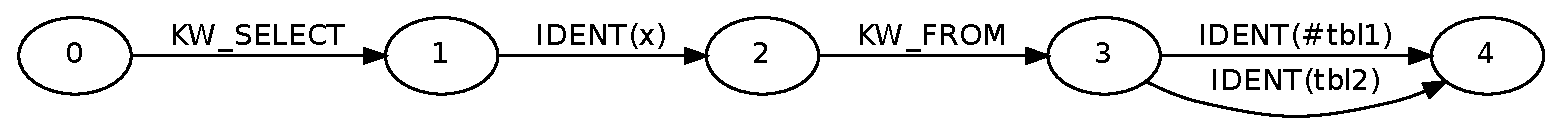
\includegraphics[scale=0.3]{Graphs/simple_sql.eps}
    \end{center}
    \caption{Foundational framework of the snork mechanism.}
    \label{fig-ffsm}
\end{figure}

Next step — abstract lexical analysis — procedure to transform input graph with string labels of edges to graph with tokens labels of edges. The result of input graph tokenization (or abstract lexing) presented in picture XXX. 

\begin{figure}
    \begin{center}
        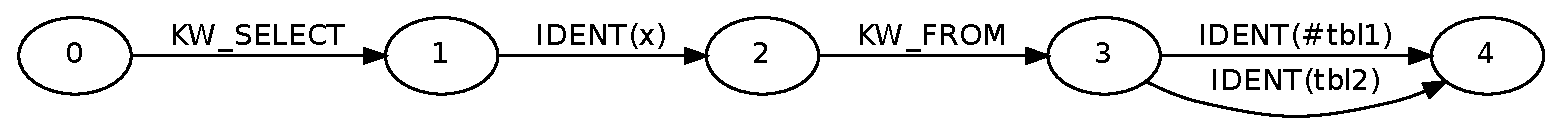
\includegraphics[scale=0.3]{Graphs/simple_sql.eps}
    \end{center}
    \caption{Foundational framework of the snork mechanism.}
    \label{fig-ffsm}
\end{figure}

Then we should perform abstract parsing. We use the second approach — reusing of classical LR parsing mechanism. Let we introduce the next example to explain basic ideas of abstract parsing. We will use the next grammar:

\begin{verbatim}
[<Start>]
s -> Ae
e -> BD | CD
\end{verbatim}

Input for analyzer builded by given grammar is a graph presented in picture VVV.

\begin{figure}
    \begin{center}
        \includegraphics[scale=0.5]{Graphs/simple_grammar_input.eps}
    \end{center}
    \caption{Foundational framework of the snork mechanism.}
    \label{fig-ffsm}
\end{figure}

The set of parser states will be computed for each graph vertice during parsing. For each vertice should be computed a parser states set which represent all states may be given during parsing all paths from sturt vertice to current (Pic 5). For example, There are 2 different states for vertice 3 in picture 5: {e-> B.D; e-> C.D}. It is a result of parsing two sequences: AB and AC. 

\begin{figure}
    \begin{center}
        \includegraphics[scale=0.5]{Graphs/simple_grammar_items.eps}
    \end{center}
    \caption{Foundational framework of the snork mechanism.}
    \label{fig-ffsm}
\end{figure}

Since the base of abstract parsing is classical LR algorithm, it is possible to process attributed grammars. So we can calculate user semantic actions. 

\subsection{Generalized LR parsing}
	Not all grammars are unambiguous but it is still necessary to process them, so there are a class of Generalized LR-analysis algorithms for ambiguous grammars handling. Classical GLR was introduced by Tomita[tomita]. It based on classical LR analysis and has the number of significant differences, which make it possible to process ambiguous grammars. Algorithm uses parse tables, which are much like as parse tables for classical LR-algorithm, but can contain more than one possible action in each cell. This situation is called conflict and can be one of the two possible types: Shift/Reduce — it is possible either shift one more token from input stream or reduce the stack — and Reduce/Reduce — there are more than one possibility to reduce the stack. Furthermore more complex data structure — Graph Structured Stack, GSS — is used instead of common stack. Manipulation with GSS is based on breadth-first search, so there are levels corresponding to the position of the token in input stream. 

Since it is possible to get more than one result of parsing in case of processing of ambiguous grammar then a special structure which allow to reuse nodes in parsing forest is used. This structure introduced by Reker[link] and named Shared Packed Parsing Forest or SPPF [ссылка?]. SPPF is an inner data structure so it can be very compact. User defined semantic which can require a lot of memory can be calculated after parsing finished only for necessary trees extracted from SPPF. This way we can reduce resources requirements. In our algorithm we also use classical GSS and SPPF as base data structures.

However classical Tomita’s GLR constraints grammar. Elizabeth Scott et al proposed development of Tomita’s idea — RNGLR-algorithm of syntactic analysis, which we will use as a base for our algorithm. RNGLR-algorithm can handle arbitrary ambiguous grammar, like classical GLR-algorithm, and it uses GSS and SPPF. They also introduced push operation instead of classical shift and goto operations, which better correspond to adding new edges to GSS [Right Nulled GLR Parsers]. So Push(k) is a type of actions (one of values of action tables) which denote that we should place symbol k to stack.  We will use this terminology hereinafter.

\subsection{Input data format}
We approximate value set by constant propagation. Resulting data structure is a graph, which has string used for expression construction on its edges and its vertices correspond to concatenations. One might say we build finite automaton describing the language which contains of dynamically generated expression values.

If loops are used in the construction of expression, value set may become infinite. We replace loops in the graph to single repetition of its body for now. This guarantee the finiteness of value set, but adversely affect the reliability of the results since this replacement can lead to both loss of some possible expression and generation of new expressions. Let consider the following example. Suppose we need to process the code below.

\begin{verbatim}
query = "select * from ";
for(int i = 0; i < tables.size(); i++)
{
if(i != 0) query += ", ";
query += tables.get(i);
}
query += ";";
\end{verbatim}

	Regular expression $”select * from ” · ({tables.get(i)}|\varepsilon) \star \cdot ”;”$ is built as a regular approximation of set of possible values of variable query. Corresponding finite automaton is presented in picture Ь. Notice, that we do not provide the value of expression {tables.get(i)} as it depends on constant propagation algorithm possibilities. In order to get rid of loop we replace it with single repetition of its body. Graph presented in picture Т is the result of the replacement for our example.


\begin{figure}
    \begin{center}
        \includegraphics[scale=0.5]{Graphs/cyclesOrig.eps}
    \end{center}
    \caption{Foundational framework of the snork mechanism.}
    \label{fig-ffsm}
\end{figure}


\begin{figure}
    \begin{center}
        \includegraphics[scale=0.5]{Graphs/cyclesApproximation.eps}
    \end{center}
    \caption{Foundational framework of the snork mechanism.}
    \label{fig-ffsm}
\end{figure}

Approximation graph does not contain paths which corresponds to values “select * from tbl1, tbl2;” and “select * from ;”. This leads to impossibility of static check of theirs correctness. Only 2 possible values of initial infinite set of values can be generated from the approximation graph. Thus we cannot check all possible values in case of loops being used to construct queries. By the way, this approach provide enough data for such problems as code highlighting because all parts of expression will be processed. 

\subsection{Graph Structured Stack}
As far as input data structure for our algorithm is DAG we can process all vertices in topological order instead  of find fix point. Stack building in classical  GLR is based on breadth-first traversal: firstly should be performed all actions with current level of stack and only when no available operation then pushes to next level will be performed. So operations in GLR stack performed level by level. In RNGLR algorithm levels corresponded with input token number. In our algorithm we define that level is a vertice number in topological order. Such definition of level allow to avoid incorrect  merging of stack’s branches. So if we want to process graph which presented in picture N then we should process vertices sequentially in the next order: 0 1 2 3 4 5 6 7. In picture M you can see the graph we want to process (picture N) layouted with levels information.

\begin{figure}
    \begin{center}
        \includegraphics[scale=0.3]{Graphs/toposort0.eps}
    \end{center}
    \caption{Foundational framework of the snork mechanism.}
    \label{fig-ffsm}
\end{figure}

\begin{figure}
    \begin{center}
        \includegraphics[scale=0.25]{Graphs/toposort1.eps}
    \end{center}
    \caption{Foundational framework of the snork mechanism.}
    \label{fig-ffsm}
\end{figure}

\subsection{Example of GSS construction}
We introduce the next example to demonstrate GSS manipulation in abstract parsing. Let we specify the next grammar of arithmetic expressions. Let only two binary operators are specified:  + and *. So, the next tokens are defined:
\begin{verbatim}
PLUS = ‘+’
MULT = ‘*’
LBR = ‘(’
RBR = ‘)’
NUM = [1..9]
\end{verbatim}

And the final grammar is:

\begin{verbatim}
s -> s PLUS e | e
e -> e MULT t | t
t -> LBR s RBR
t -> NUM
\end{verbatim}

Input graph to process presented in picture <<H>>. This graph ready to parsing: vertices are numbered in topological order and edges labels are tokens. This graph is a representation of the next set of arithmetic expressions:

\begin{equation}
\begin{split}
\{ \\
1+4*(7*8) (path 0-1-2-3-8-9-10-11-12-13) \\
1*5+(7*8) (path 0-1-4-5-8-9-10-11-12-13) \\
1+6+(7*8) (path 0-1-6-7-8-9-10-11-12-13) \\
\}
\end{split}
\end{equation}

\begin{figure*}
    \begin{center}
        \includegraphics[scale=0.4]{Graphs/input1.eps}
    \end{center}
    \caption{Foundational framework of the snork mechanism.}
    \label{fig-ffsm}
\end{figure*}

Now we can show stack transformations performed during analysis of the graph presented in picture <<H>> At the start stack contains only one start vertice with number 0. At the first step token NUM from edge 0--1 is pushed. After that the sequence of reductions is performed. The reduction to nonterminal s is final. Note that all intermediate outcome should be saved in stack because pushes to next level may be available for all produced states.  In our example MULT from edge 1--4 can be pushed for state corresponded with vertice with id=1 and PLUS from edges 1--2 and 1--6 can be pushed for state corresponded with vertice with id=18. On the other hand there are no pushes for vertices with id=21 and id=17 and this vertices and outgoing edges will be removed at the next step. Stack after described operations presented in picture <<PP>>

\begin{figure}
    \begin{center}
        \includegraphics[scale=0.65]{Graphs/stack_1_2.eps}
    \end{center}
    \caption{Foundational framework of the snork mechanism.}
    \label{fig-ffsm}
\end{figure}

At the next step we should process all outgoing edges for vertice with id=1 in input graph. This vertice has 3 outgoing edges and pushes for all of them should be constructed. But only one of pushes should be available for further processing: corresponded with vertice with minimal number. Postponed pushes will be processed in order of topological number of its start vertice. In our example each branch will be sequentially processed to vertice with id=8 than the next branch will be restored from postponed pushes and processed. Stacks corresponded with processing of the paths 1-2-3-8 and 1-4-5-8  are presented in pictures TTT--TTTT. Note that in the pictures TTT+1 — TTTT postponed pushes are not draw.

\begin{figure}
    \begin{center}
        \includegraphics[scale=0.65]{Graphs/stack_1_3_m.eps}
    \end{center}
    \caption{Foundational framework of the snork mechanism.}
    \label{fig-ffsm}
\end{figure}

\begin{figure}
    \begin{center}
        \includegraphics[scale=0.6]{Graphs/stack_1_4.eps}
    \end{center}
    \caption{Foundational framework of the snork mechanism.}
    \label{fig-ffsm}
\end{figure}

\begin{figure}
    \begin{center}
        \includegraphics[scale=0.6]{Graphs/stack_1_6.eps}
    \end{center}
    \caption{Foundational framework of the snork mechanism.}
    \label{fig-ffsm}
\end{figure}

We get the stack presented in picture M when all edges incoming to vertice with id=8 are processed. There are 3 incoming edges for vertice 8 but as you can see that only 2 top vertices in stack are merged. It is happens because only 2 of 3 corresponds with identical parsing states.  After that, when open brace form edge 8--9 in input graph will be processed, all vertices corresponds with identical states and can be merged. Result of merge presented in picture M+1

\begin{figure}[h]
    \begin{center}
        \includegraphics[scale=0.4]{Graphs/stack_4_9.eps}
    \end{center}
    \caption{Foundational framework of the snork mechanism.}
    \label{fig-ffsm}
\end{figure}

\begin{figure}
    \begin{center}
        \includegraphics[scale=0.3]{Graphs/stack_4_10.eps}
    \end{center}
    \caption{Foundational framework of the snork mechanism.}
    \label{fig-ffsm}
\end{figure}

Further changes in stack will be performed in order of algorithm described above. In picture MM you can see the final state of GSS.

\begin{figure*}
    \begin{center}
        \includegraphics[scale=0.5]{Graphs/stack_5_13.eps}
    \end{center}
    \caption{Foundational framework of the snork mechanism.}
    \label{fig-ffsm}
\end{figure*}

	In this example we demonstrate main steps of GSS construction: branching, pushes processing, branches mering. You can see that it is similar to classical GLR GSS but with some changes in pushes processing. 


\subsection{Shared Packed Parsing Forest}
	Lightweight inner representation of parsing results — Shared Packed Parse Forest, SPPF — was proposed in paper [Rekers] in order to minimize the size of parsing forest. After parsing is completed SPPF can be used for semantics calculation. User can choose one parsing tree and calculate semantics for it only, which can help to get rid of redundant calculation. Part of the calculation can also become redundant if it took place in the erroneous stack branch. These features are very valuable for abstract analysis, as the number of common nodes in parse trees are huge and using SPPF one can reuse them among trees, corresponded to different paths in input graph. The number of mistakes can also be enormous and there is no need to calculate semantics for the whole parse forest. Use of SPPF can significantly speed up abstract analysis and reduce memory consumption. 

SPPF building in the process of abstract analysis does not differ from the one in RNGLR-algorithm. Intermediate nodes are introduced for correct representation of multiple possible parse trees for nonterminal being processed. In our algorithm if there are several ways to construct node for nonterminal S, then additional vertices are created as its children and each of them is a root of parse tree for one of the possibilities. We paint nodes for such nonterminals in red in our pictures.  In the picture Р you can see a root node S which has 3 different variants for tree. Child nodes of node S with label prod0 is additional nodes. Subtrees of them are possible variants of s. 

As the process of SPPF construction is the same as in classic RNGLR-algorithm, we just provide the result for the example being described above.

\begin{figure}
    \begin{center}
        \includegraphics[scale=0.3]{Graphs/ast.eps}
    \end{center}
    \caption{Foundational framework of the snork mechanism.}
    \label{fig-ffsm}
\end{figure}

As it was said before, sometimes there is no need to calculate the semantics for the whole parse forest, or the forest is too large. It is also possible that there are trees which are correct syntactically but not semantically . In these cases lazy tree generation can help to avoid unnecessary semantics calculation. This way one can retrieve trees from SPPF and calculate semantics for them one-by-one.  

\subsection{Parsing Tables}
Abstract parsing use original LR parsing tables. Kyung-Goo Doh, Hyunha Kim and David A. Schmid in their works use LALR(1) tables generated with camlyacc[footnote]. In our tool we use RNGLR parsing algorithm which can process arbitrary context free grammars, and was proposed by Elizabeth Scott and Adrian Jonstone. This algorithm was implemented as part of YaccConstructor. Different dialects of SQL with procedure extensions JavaScript or other languages can be used as embedded languages. Available specification of this languages often is not LALR(1) and contains ambiguity.  So it is important to have ability to process arbitrary context-free grammars in order to simplify development and support of language processing tools. Therefore using of GLR parsing algorithm is better than LALR(1) and our algorithm of abstract parsing use original RNGLR parsing tables. 

\section{Evaluation}
Generator of abstract parsers based on described parsing algorithm was implemented in F\#[FS] programming language as a part of research project YaccConstructor[YC]. RNGLR parsers generator which is used as base of our algorithm was implemented before as a part of YaccConstructor. As we discussed generator is reused without any changes. Table interpreter was modified, however main data structures and core of logic were reused. Implemented tool can generate tool usable for abstract parsing of specific language was specified in input grammar  like classical parser generator. Abstract lexer generator and approximation builder were implemented also. General high level structure of our tool presented in picture X.

\begin{figure}
    \begin{center}
        \includegraphics[scale=0.25]{Graphs/General_structure_of_generator.eps}
    \end{center}
    \caption{Abstract analysis tool structure.}
    \label{fig-ffsm}
\end{figure}

We compare generated parser with similar tools in order to estimate its efficiency. Only Alvor is available for comparison at this moment. Tool developed by Kyung-Goo Doh with team and described in their papers is also very interesting and important for comparison but neither sources nor binaries of this tool are available.

Grammar of the subset of Transact SQL language was developed for  testing purposes. Grammar contains description of procedure extension and Data Manipulation Language. The grammar developed is available in project repository[YCRepo]. We want to test parser only so approximation building was omitted. So input data is a set of previously generated and serialized representations of dynamic expression approximations. We have used our experience in production information system migration  from MS-SQL Server 2005 to Oracle 11gR2 to generate relevant input data. The source system consists of 850 stored procedures and contains more than 3000 dynamic queries. Total size of migrated system is 2,7 million lines of code. The number of operations to construct values of more than half of queries is between 7 and 212 and average is 40. As a result of information system source code analysis we found that the most frequent template of dynamic query building is sequential concatenation of blocks constructed with branching operators: if statement or case statement. Input data for tests were generated in order to present dynamic expressions which may be builded by the most popular way we detected. As a result, each test is described by two parameters: the number of parallel edges in each block m and the number of sequentially concatenated blocks n. All blocks in one sequence have equal number of parallel edges. Example of graph with m = 2 and n = 2 is presented in picture Y.

\begin{figure}
    \begin{center}
        \includegraphics[scale=0.5]{Graphs/x_10.eps}
    \end{center}
    \caption{Foundational framework of the snork mechanism.}
    \label{fig-ffsm}
\end{figure}

Structure of input data was identical for all tested tools but representation of data is different for tolls and we should apply it in tests generator. YaccConstructor uses graph as an input data structure and loads data from DOT[footnote] file. Alvor, on the other hand, uses regular expression corresponded to finite automaton which was represented as a graph for YaccConstructor and load it from text file. The following constructions are available:

\begin{itemize}
\item “a” “b” — concatenation
\item  {“a”, “b”, “c”} — variants
\end{itemize}

	We created a test set generator which used patterns provided and generated tests for both YaccConstructor and Alvor. Input regular expression for Alvor and the equivalent input graph for YaccConstructor are presented in picture Y and X.
We used PC with configuration presented below for test purposes.

\begin{itemize}
    \item Operation system: Windows 8.1 Pro
    \item Operation system type: 64-bit OS, x64-based CPU
    \item CPU: Intel Core i7-2620M CPU 2.70GHz
    \item RAM: 12Gb
    \item Considering tools were implemented for different platforms (Alvor for Java platform, YaccConstructor for .Net framework) we used corresponding environments:
        \begin{itemize}
        \item Java: 
            \begin{itemize}
                \item Java(TM) SE Runtime Environment (build \verb|1.7.0_45-b18|)
                \item Java HotSpot(TM) 64-Bit Server VM (build 24.45-b08, mixed mode)
            \end{itemize}
        \item .Net:
            \begin{itemize}
                \item Runtime  4.0
            \end{itemize}
        \end{itemize}
\end{itemize}

You can find the set of diagrams which illustrate result of performance measurement for YaccConstructor and Alvor.

\begin{figure}
    \begin{center}
        \includegraphics[scale=0.65]{Graphics/m1.eps}
    \end{center}
    \caption{Foundational framework of the snork mechanism.}
    \label{fig-ffsm}
\end{figure}

\begin{figure}
    \begin{center}
        \includegraphics[scale=0.65]{Graphics/m2.eps}
    \end{center}
    \caption{Foundational framework of the snork mechanism.}
    \label{fig-ffsm}
\end{figure}

\begin{figure}
    \begin{center}
        \includegraphics[scale=0.65]{Graphics/m3.eps}
    \end{center}
    \caption{Foundational framework of the snork mechanism.}
    \label{fig-ffsm}
\end{figure}

\begin{figure}
    \begin{center}
        \includegraphics[scale=0.65]{Graphics/yc.eps}
    \end{center}
    \caption{Foundational framework of the snork mechanism.}
    \label{fig-ffsm}
\end{figure}

\begin{figure}
    \begin{center}
        \includegraphics[scale=0.65]{Graphics/alvor.eps}
    \end{center}
    \caption{Foundational framework of the snork mechanism.}
    \label{fig-ffsm}
\end{figure}


From the data gathered it can be concluded that the performance of implemented tool is better than performance of Alvor in a wide rage of practical cases: 2 -- 3 parallel edges in block and the number of blocks up to 200. By the way, in case of linear input our tool is worse than Alvor.

\section{Future work}
One of the main application of developed tool is errors detecting. So improvements of corresponded algorithms is very important. Error reporting and error recovery in generalized LR parsing are nontrivial problems. A considerable amount of research has been done on improving the error reporting for LR parsers, relatively little work has been done for GLR parsers.[обзор GLR-ов]. During the experiments we found out that error processing in GLR-based abstract parsing is far more complex than in classical  GLR parsing algorithm. It is caused by increased algorithm complexity. On the other hand error processing in LL parsing algorithm may be easier than in LR, so we plan to investigate GLL parsing algorithm and research an ability to use it as a base for abstract parsing. We expect that GLL-based abstract parsing will be based on the same ideas as GLR-based because it also manipulate with GSS and SPPF data structures. Also we hope that error processing in GLL-based abstract parsing will be simpler and more qualitative.

In spite of problems with error processing GLR-based abstract parsing algorithm may be useful in situations when it is necessary to process a huge amount of code which should be mainly correct in a short time. Such situations often occur in software reengineering. It is important that in such case we may notify developers about all suspicious situations in code. Migration to generalized parsing algorithms with better performance than RNGLR -- BRNGLR or RIGLR -- may help to increase performance of abstract parsing.

It is important to improve quality of analysis so the next big task is improvement and  adjustment of approximation. Firstly it is necessary to support cycles in input graph. This changes may provoke parsing complexity increase and performance problems. It is possible to apply improved algorithm only if input graph contain cycles to solve this problems. Our current experience of real world information systems processing shows that cycles are not very popular to construct dynamic expressions.



\appendix
\section{Appendix Title}

This is the text of the appendix, if you need one.

\acks

Acknowledgments, if needed.

% We recommend abbrvnat bibliography style.

\bibliographystyle{abbrvnat}

% The bibliography should be embedded for final submission.

\begin{thebibliography}{}
\softraggedright

\bibitem[Smith et~al.(2009)Smith, Jones]{smith02}
P. Q. Smith, and X. Y. Jones. ...reference text...

\bibitem[Smith et~al.(2009)Smith, Jones]{smith03}
P. Q. Smith, and X. Y. Jones. ...reference text...

\bibitem[Smith et~al.(2009)Smith, Jones]{smith04}
P. Q. Smith, and X. Y. Jones. ...reference text...

\bibitem[Smith et~al.(2009)Smith, Jones]{smith05}
P. Q. Smith, and X. Y. Jones. ...reference text...

\bibitem[Smith et~al.(2009)Smith, Jones]{smith06}
P. Q. Smith, and X. Y. Jones. ...reference text...

\bibitem[Smith et~al.(2009)Smith, Jones]{smith07}
P. Q. Smith, and X. Y. Jones. ...reference text...

\bibitem[Smith et~al.(2009)Smith, Jones]{smith08}
P. Q. Smith, and X. Y. Jones. ...reference text...

\end{thebibliography}


\end{document}


